\documentclass{report}
\usepackage[utf8]{inputenc}
\usepackage{xcolor}
\usepackage{url}
\usepackage[nottoc]{tocbibind}
\usepackage{graphicx}
\usepackage[bottom]{footmisc}
\usepackage{cite}
\usepackage{caption}
\usepackage{subcaption}
\usepackage{listings}
\usepackage[safe]{tipa}
\usepackage{ucs}
\usepackage[utf8x]{inputenc}
\usepackage[T1]{fontenc}
\usepackage{upgreek}
\usepackage[shortlabels]{enumitem}
\bibliographystyle{ieeetr}

\definecolor{codegreen}{rgb}{0,0.6,0}
\definecolor{codegray}{rgb}{0.5,0.5,0.5}
\definecolor{codepurple}{rgb}{0.58,0,0.82}
\definecolor{backcolour}{rgb}{0.95,0.95,0.92}


\lstdefinestyle{mystyle}{
    backgroundcolor=\color{backcolour},   
    commentstyle=\color{codegreen},
    keywordstyle=\color{magenta},
    numberstyle=\tiny\color{codegray},
    stringstyle=\color{codepurple},
    basicstyle=\ttfamily\footnotesize,
    breakatwhitespace=false,         
    breaklines=true,                 
    captionpos=b,                    
    keepspaces=true,                 
    % numbers=left,                    
    % numbersep=2pt,                  
    showspaces=false,                
    showstringspaces=false,
    showtabs=false,                  
    tabsize=2
}


\title{Project Document: Deep(FAMS)}
\author{Mohammad Alyetama \\
Ali Al-Ramini \\
Fangyi Li }
\date{}

\begin{document}

\maketitle

\tableofcontents

\begin{abstract}
This project will attempt to optimize generative adversarial networks to generate good results with limited data using a recently proposed mechanism, the adaptive discriminator augmentation (ADA). This project aims to evaluate the reproducibility and generalizability of the results generated by this proposed mechanism. Since the ADA does not require changes to the network architectures, we will build models based on the StyleGAN2 and test it to evaluate the reported results' reproducibility in the original paper. Using several small datasets, we follow the code provided in the paper, except for some tiny changes, like resizing image of datasets to increase the feasibility considering the GPU we have; and we plan to demonstrate that the ADA produces good results using those limited training images.
\end{abstract}

\chapter{Milestone 1: Project Ideas}

\section{Introduction}

\subsection{Project Idea 1}

Generative adversarial networks always seek to increase the dataset size to generate desirable results as an approach to generative modeling. The massive demand for data is challenging to lots of areas, and thus placing constraints on more widely being used of this practical approach. However, the dataset size reduction can cause overfitting issues in checking step by discriminator sub-model. Applying dataset augmentation can generate the augmented distribution, which is highly undesirable to generate samples.
An attempt to apply a wide range of augmentation by Kerras et al. is trying to demonstrate GAN can use a smaller dataset size but prevent the augmentation `leaking` at the same time. In this project, we will follow Karras et al. methods of adaptive discriminator augmentation mechanism~\cite{karras2020training} to try to reproduce their result.


\subsection{Project Idea 2}
There is a great interest in improving the cycling infrastructure in Nebraska by analyzing cyclic data. Toward this goal, we acquired the Strava Metro data covering Nebraska's state from January 2017 to December 2019.  Strava provides data into four categories edges, nodes, origin-destination polygons, and shapefiles that contain spatial attributes to create maps using GIS software. Edges are street segments between nodes. In other words, a set of edges form a street. Nodes are the intersections between edges, and origin-destination polygons divide a space into smaller areas. Every category of Strava data is divided into yearly, monthly, and hourly data. The Strava data, made available by the social fitness network company Strava, includes raw data for the hour-by-hour counts for bicycle trips that have been mostly incorporated into existing maps for better visualization. In this project, we propose building a deep learning regression model that utilizes Strava data in addition to weather data to predict the number of cycling trips in Nebraska. 

\section{Project Idea 1: Evaluating the Reproducibility of Training GAN With Limited Data}

Generative adversarial networks (GAN) is a generative modeling approach that uses deep learning techniques to automatically discover and learn the input patterns to generate an output that would plausibly appear as if it was sampled from the original input data~\cite{goodfellow2014generative}. For example, a GAN that uses convolutional neural networks (CNNs) can take pictures of humans as input data and generate new pictures of humans with plausible characteristics that look superficially genuine. This approach gained popularity after it was introduced by Goodfellow and his colleagues in 2014~\cite{goodfellow2014generative}. In their paper, they describe GAN as a structure with two essential sub-models: (1) a generator model that learns to generate superficially plausible data, which the discriminator takes as negative training examples, and (2) a discriminator model that learns to discriminate between generated and real data, and penalizes the generator if an implausible result is detected~\cite{creswell2018generative}. The generator and the discriminator are neural networks that are directly connected. This connection allows the discriminator to send a signal, through backpropagation, that the generator uses to update its weights. Specifically, the generator samples a vector that is randomly drawn from a Gaussian distribution and use it to seed its generative process and match it to a distribution of interest, creating a `latent space.` With sufficient training, the generator model can learn the input data's statistical latent space and create output data similar to what is observed in the input data~\cite{radford2015unsupervised}. An example of such data is then processed by the discriminator model and attempt to distinguish it from the real distribution of the data (i.e., a binary class of fake/real). The generator model's goal here is to maximize the error of the discriminator model. In other words, the generator model becomes more effective the more the discriminator process fake data as real data. The GAN approach has been used in fashion, science, and video games with impressive results~\cite{gui2020review}.

However, a significant challenge in this area is the large number of data required to build a good GAN model, which is in some cases not available for researchers interested in applying GAN to their research question. GAN typically requires a large dataset because, with smaller datasets, the discriminator model ends up overfitting to training data examples, and the training eventually diverges~\cite{zhao2020improved}. While dataset augmentation is typically applied in such situations to solve overfitting~\cite{shorten2019survey}, it cannot achieve this in GAN models. The inability to solve this problem with dataset augmentation stems from GAN's ability to employ this technique without learning the augmented distribution and leaking these results to the model~\cite{zhao2020improved} causing undesirable outcomes. Therefore, the challenge is to demonstrate that GAN can be used with smaller datasets without the pitfalls mentioned above.

A recent attempt to solve this problem was proposed by Kerras et al.~\cite{karras2020training}, demonstrating that it is possible to obtain good results using limited data. The critical point in their proposed approach is that we can prevent overfitting and augmentations leak by applying a wide variety of augmentation methods. Their work demonstrates the validity of their approach by describing a set of conditions that allows controlling the augmentations leak problem and then proposes an adaptive discriminator augmentation pipeline that can dynamically control the strength of the augmentation. This is a novel approach they propose contrasting the convention of tuning the augmentation strength manually, a resources-consuming process. The process of building an adaptive discriminator augmentation mechanism, as described by the authors, is achieved by 
(a) Declare an overfitting heuristic, r, in which a value of zero represents no overfitting and a value of 1 means perfect overfitting.
(b) Adjust augmentation probability (\textit{p}) until the heuristic reaches a target value, which in turn can be processed by:
(1) initializing the augmentation strength to zero, then adjusting p every four mini-batches based on an overfitting heuristic (\textit{rf}).
(2) if \textit{rf} shows too much overfitting, it is countered by a fixed increment of \textit{p} (or fixed decrement if \textit{rf} shows too little overfitting).
(3) The adjustment size is then set in a way that allows p to quickly rise from 0 to 1 while clamping p after every step from below to zero (adaptive).
(4) The results from adaptive versus fixed \textit{p} are then compared.
Using such mechanisms on limited data, the authors demonstrated that their adaptive discriminator augmentation approach improved the quality of the result and stabilized training with a minimal effect on resources consumption, showing that their strategy is both viable and cost-efficient~\cite{karras2020training}.


In this project, we will attempt to reproduce the results reported by Karras et al. using their adaptive discriminator augmentation mechanism. We expect our reproduced work to support Kerras et al.'s claim made in the paper; that is, good results can be obtained in a GAN model with only a few thousand training images. The original article's hypothesis was tested using five small datasets (METFACES, BRECAHAD, AFHQ, and CIFAR-10). Here, we plan to test adaptive discriminator augmentation on additional datasets to find out whether the scope of Kerras et al. paper is generalizable. This would be a pivotal point in our project because the authors of the article claim that their model's strength stems from its ability to work despite variations between datasets in content and size. This is a central argument to their approach. They experimentally demonstrate that a set of fixed augmentation parameters (as opposed to adaptive parameters) will miss the utmost advantage a GAN model can achieve. Overall, our results will allow us to evaluate the reproducibility of the results, the readability of the source code, and experiment with the ability to generalize the approach described in the paper with different datasets.



\section{Project Idea 2: Using App Data to Model Bicycling Patterns in Nebraska}

Across the United States, cycling is becoming increasingly popular as users shift travel modes amid concerns of health, physical activity, air, and environmental quality, and to escape roadway congestion. Unfortunately, the infrastructure in the U.S. traditionally caters to automobile traffic creating impediments for bikers and impacting their safety. To accommodate cycling, a major challenge is the lack of machine learning model representation of the available data to assess the attributes of present assets accurately and to inform additional investments to integrate bicycles into our transportation system. Toward that end, this project uses citywide bicycle travel data (i.e., Strava Metro Data) to provide a comprehensive description of daily cycling in a mid-size American state as a proof-of-concept approach to planning for cycling. 
\\Various governments and organizations utilize big data to evaluate their cycling infrastructure ~\cite{hall2012open}. Big cycling data are usually collected using live point data, journey data, Bike-Share Programs (BSP), and GPS. Live point data are collected on intersections using cameras on traffic lights, counting stations, or even sensors. While the journey data provide information about the origin and the destination of the trip, it does not provide the trip details. This set of data could be collected from BSP or by other sources like online questionnaires. BSP data are complete and in real-time. However, these data only give information within the area of its location ~\cite{ romanillos2016big, rogers2000counting}. Strava is considered a GPS program that is made available by the social fitness network company Strava. Strava utilizes the Open Street Map (OSM) to deliver its data. These GPS data are very detailed and historical but represent a small sample of the cyclists' total population.  
Strava app data contains a vast amount of spatial and temporal details to predict cycling activity patterns. It provides a good approximation of the most-used routes and the peak months and hours. To protect privacy, the Strava data set is combined into population datasets. While a small portion of cyclic may use Strava to log their trips or the app might track trips for users using other transportation methods ~\cite{hall2012open, romanillos2016big, fishman2016cycling }, several studies showed that there is a strong correlation between the Strava data and the ground-truth data obtained from counting stations ~\cite{hong2020evaluation, jestico2016mapping}. 
Cycling is affected by several factors such as weather, time of the day, infrastructure, congestion, environment, income, public transportation, health, population density, the slope of the street, and cultural view towards cycling ~\cite{musakwa2016mapping, roy2019correcting, hochmair2019estimating}. But traditionally, access to high-quality data has limited our understanding of cycling behavior and route choice in the face of these myriad factors. In this project, we explore the weather effects and weather parameters sensitivity to cycling in Nebraska. This work aims to specify cycling behavior further as it relates to specific factors, but more importantly, to determine the quality of the specified factors in determining the number of cycling trips over a vast area like the State of Nebraska. 
Using data visualization techniques and Deep learning regression (e.g., ANN, RNN, LSTM, and GRU)~\cite{hassoun1995fundamentals, graves2013generating} we study the most influential time-related factors affecting the cycling patterns in Nebraska. Moreover, cycling is usually categorized into two classes, commuting and recreational. The proposed study will take advantage of the data shared by Strava to predict the number of commutes and recreational activities across all streets. 

\section{Conclusions}
\subsection{Project Idea 1}
The core of this project is to test if the methods proposed by Karras et al. can solve the problem of augmentation leak and then ease the burden of huge datasets required by GAN. Given that the proposed mechanism is relatively new and paradigm-shifting, we believe that the idea of reproducing the paper's results would be greatly valuable. Studying such an approach to solve overfitting and subsequent problems while using limited datasets in GAN allows any researcher access to cost-efficient models.

\subsection{Project Idea 2}
This project provides an exciting idea: to create a deep learning model that predicts Nebraska's cycling patterns. With the help of high-quality data sources (e.g., Strava Data and Weather Data), this project's outcomes could be essential towards understanding how cyclists react to temporal variations. However, the spatial factors affecting cycling should also be studied, adding more complexity to the problem. The spatial representation of the data could be tough to map during this short period. Additionally, this idea is essential considering the current situation with COVID-19, adding more complexity and difficulty to reproducing the analysis to agree with the latest status.


\chapter{Milestone 2: Project Selection}

%In this chapter, you should select your project, formally define it, and propose two approaches, each with a work plan.  You should follow The Heilmeier Catechism~\cite{heilmeier}, which is a set of questions used to evaluate proposed research programs:  
%\begin{enumerate}
   % \item What are you trying to do? Articulate your objectives using absolutely no jargon.
   %\item How is it done today, and what are the limits of current practice?
   %\item What is new in your approach, and why do you think it will be successful?
   %\item Who cares? If you are successful, what difference will it make?
   %\item What are the risks?
   %\item How much will it cost?
   %\item How long will it take?
   %\item What are the mid-term and final ``exams'' to check for success?
%\end{enumerate}

\section{Introduction}

Our group semester project is Evaluating the Reproducibility of Training GAN with Limited Data.
As mentioned in the last chapter, GAN, representing Generative Adversarial Networks, is a generative modeling approach using deep learning techniques to automatically discover and learn the input patterns to generate an output that would plausibly appear as it was sampled from the original dataset\cite{goodfellow2014generative}. The GAN approach has gained its popularity in diverse areas including but not limited to fashion, science, and video games\cite{gui2020review}. The success of the GAN approach can be attributed to its structure: a generator model and discriminator model connecting, where the generator model learns to generate superficially plausible data, and the discriminator model takes the generated data to discriminate with the real data and penalizes the generator if there’s an implausible result detected\cite{creswell2018generative}. The connection between the two models allows the updating of the generator based on the discrimination of discriminator and generating the more plausible outputs\cite{radford2015unsupervised}. However, its success is still weakened by the challenge of its need for the large dataset to ensure the GAN approach's efficiency. The applying of a small dataset makes the discriminator ended up overfitting to training data examples, and the training diverged\cite{zhao2020improved}.
What’s more, if the augmentation of the dataset is introduced to resolve the overfitting, the augmented distribution can be caused, which is highly undesirable for sample generation.\cite{zhao2020improved} Therefore, it is a challenge that applying the GAN approach with the smaller dataset and avoid the mentioned pitfalls at the same time. In the research by Kerras et al. \cite{karras2020training}, one method was come up to realize obtaining good results using a smaller dataset. The research was applying a wide variety of augmentation methods. The results demonstrated the validity by describing conditions that control the augmentations leak problem and then proposed an adaptive discriminator augmentation pipeline that can control the strength of the augmentation. 

The paper provides a small dataset to obtain good results from the GAN approach; this possibility is valuable since the broke of dataset size limitation will help the GAN approach spread in more areas, and correspondingly those areas will obtain an efficient way to solve their problems. 
The offered methods provide us with the prospect for similar problems, which is an excellent chance for us to learn about model learning. Additionally, the decision on Evaluating the Reproducibility of Training GAN with Limited Data is also the result of considering the feasibility within the limited one-semester timeline.


\section{Problem Specification}

%Formally define your chosen problem, including the following, as subsections:
%\begin{enumerate}
%    \item A brief statement of your project topic (HC1).
%    \item Motivation for your topic: why it is important and exciting (HC3, HC4). If your work is in an application area, be careful to avoid technical jargon from that area that is outside of computer science. If you must use a term, define it as carefully and simply as possible.
%   \item What resources will you need, including data sets and libraries that need to be installed on {\tt crane} (HC6).
%   \item Cite at least three references (at least two published journal or conference papers) (HC2).
%\end{enumerate}

The work presented in this project provides a complete evaluation of the proposed generative image training models by Karras et al. in\cite{karras2020training}. The idea is to reproduce the generative image models trained on significantly fewer data than other approaches in the past. We are going to use the adaptive discriminator augmentation mechanism proposed in the paper, following the codes provided in\cite{karras2020training}, to assess its reproducibility and ability to classify relatively small (few thousands) datasets.\\


In many application fields, it is challenging to collect large datasets to perform data training. For example, in medicine, there is an ongoing challenge in modeling the possible appearance of biological specimens (tissues, tumors, etc.) This is a growing body of research that seems to suffer from limited high-quality data constantly. As introduced above, GAN has a great performance in training unlimited online data\cite{goodfellow2014generative, miyato2018cgans, miyato2018spectral, brock2018large, karras2017progressive, karras2019style, karras2020analyzing}, as a result, it cannot be used for lots of specific applications that only collected around hundreds or thousands of samples, where collecting more samples can be very complicated and costly. If the small datasets are applied for the GAN approach, the overfitting will occur in the discriminator. The dataset augmentation always used for overfitting can lead to training divergence in this GAN approach situation, which will not get a good result in the end. The method proposed by Kerras et al. has been providing the chance to break this deadlock. To make the GAN approach more suitable for small datasets, this method makes use of a wide range of augmentations to ensure that the discriminator does not overfit while the generator does not also leak. This method's success will make the GAN approach more available for those specific applications with relatively small datasets, where's great potential to solve more problems. Thus, in this project, we evaluate the GAN augmentations proposed by Karras et al. and reproduce their approaches in terms of model architecture and code. Moreover, we test the model on several additional small datasets and compare our results with the original paper authors' results to find out if the scope of the model is generalizable. From an applied point of view, this work contributes to efficiency; by testing the GAN augmentations proposed, this work will further confirm the elimination of the barrier for applying GAN-type
models in many applied fields of research. \\

In this project, there are some requirements mentioned in the original paper to make sure reproduce the study successfully:
\begin{itemize}
\item Python 3.7
    \item TensorFlow 1.14 to develop and train ML models.
    \item \texttt{Numpy>=1.14.3 for working with arrays.}
    \item \texttt{tensorflow\_ds and pandas>=1.0 to load datasets.}
    \item High-end NVIDIA GPUs with at least 12 GB of GPU memory, NVIDIA drivers, CUDA 10.0 toolkit and cuDNN 7.5.
\end{itemize}



We will use several datasets that consist of a limited number of training images, including: 
\begin{enumerate}
\item METFACES\cite{karras2020training} 
\item AFHQ\cite{choi2020stargan}
\item CIFAR-10\cite{krizhevsky2009learning}
\item StandfordDogs\cite{KhoslaYaoJayadevaprakashFeiFei_FGVC2011, imagenet_cvpr09}
\item Cars196\cite{KrauseStarkDengFei-Fei_3DRR2013}
\item OxfordFlowers102\cite{Nilsback08}
\end{enumerate}


\section{Proposed Method:}

%%%%%%%%%%%%%%%%%%%%%%%%%%%%%%%%%%%%%%%%%
%Propose a step-by-step approach to solve your chosen problem.  You should include 
%a precise work plan: what you plan to do, what data sets you will test on, how you will preprocess the data, what the steps (pipeline) of this method (e.g., what NN architecture(s) will be used and how they'll be linked), how you will evaluate performance, what is your timeline, etc.\ (HC5, HC7, HC8).  One or more of your references should relate to aspects of this. 
%%%%%%%%%%%%%%%%%%%%%%%%%%%%%%%%%%%%%%

In this section, since we are attempting to reproduce an article that proposes one specific method, we provide extended details for this one method.

\begin{itemize}
    \item \textbf{Datasets.} In our experiments, we will use three out of the six datasets used in the original paper. That is, {\tt METFACES}, the Animal Faces-HQ ({\tt AFHQ}) dataset, and {\tt CIFAR-10}. In addition to these three datasets, we will test the generalizability of the original paper's findings by using three other small datasets that were not tested in Keras et al. paper. These are the {\tt StanfordDogs} dataset, the {\tt Cars196} dataset, and the {\tt OxfordFlowers102} dataset. See Table 1 for more details about the datasets we plan to use in the present project. The datasets will be either downloaded from Tensorflow datasets collection (CIFAR-10, Cars196, OxfordFlowers102, and StanfordDogs) or from source (AFHQ and METFACES).
    
    \begin{table}[!ht]

        \centering 
        \caption{Datasets Information}
        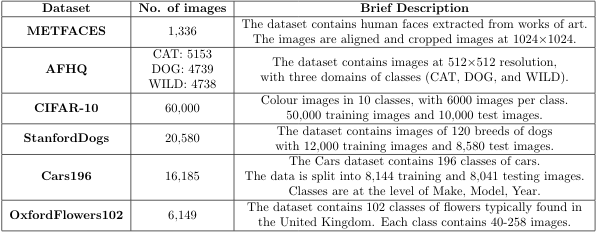
\includegraphics[width=1\textwidth]{figs/table_1.png}
    \end{table}

    
    \item \textbf{Preprocessing.} The {\tt METFACES} dataset is available in both raw and process format. We will use the raw format and process it by aligning and cropping images at $1024 \times $1024 pixels, then use various automatic filters to prune the dataset. The {\tt AFHQ} dataset will be split into three subsets: CAT, DOG, and WILD. All datasets will be standardized to make the training faster and reduce the probability of getting stuck in local optima.
    
    \item \textbf{Pipeline}.
    The authors of the paper implemented their techniques on top of the {\tt StyleGAN2} official TensorFlow implementation and kept most of the network architecture unchanged.  For this project, we will use the baseline StyleGAN2 as illustrated in Figure 2.1.\\
    
    \begin{figure}[!ht]
    \centering 
    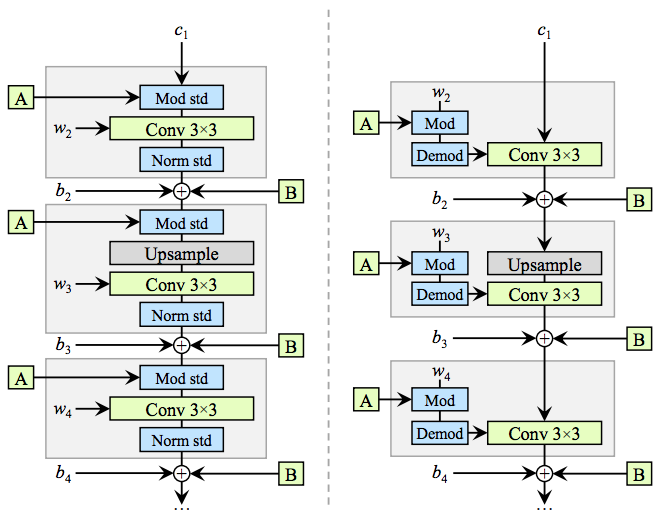
\includegraphics[width=1\textwidth]{figs/stylegan2_arch.png}
    \caption{StyleGAN2 architecture}
    \end{figure}


    \begin{enumerate}
        \item \textbf{\textit{The generator model.}} The generator model starts with an input layer that takes an image as input and a vector as an output in the latent space and gets normalized. We follow this with two fully connected layers (Dense layers), then we add a 4×4 convolutional layer, upsample, a $4 \times $4 ToRGB layer, then a UpConv layer (upsampling + Sum + Residual Unit). We repeat this six more times while increasing the kernel size to the power of 2 ($8 \times $8, $16 \times $16, $32 \times $32, etc.). 
        
        \item \textbf{\textit{The discriminator model.}} For the discriminator model, following the input layer, we will add a FromRGB layer with a kernel size of $256 \times $256, followed by a DownConv layer (convolutional layer + Residual Unit + downsampling), a skip connection. We will repeat this six times before adding a mini-batch standard deviation, a convolutional layer then a fully connected layer.
        
        \item \textbf{\textit{Quality metrics.}} In this project, we will use multiple metrics to evaluate the performance of our GANS.\\We will compute Frechet Inception Distance (FID) against the full dataset for each network to evaluate it. FID is a metric that calculates the distance between feature vectors calculated for real and generated images. Low FID score indicates that the images generated by the generator is similar to the real ones. We expect the FID result to be minimumal and comparable to results from the original paper (5.59 to 2.42). To calculate FID, we will perform the following:
                \begin{enumerate}[(a)]
                \item Use the Inception v3 pre-trained model and extract the feature vectors of real and generated images.
                \item Find the mean feature-wise of the vectors generated in the previous step.
                \item Generate the feature vectors' covariance matrices.
                \item Calculate the sum of the elements along the main diagonal of the square matrix.
                \item Calculate the squared difference of the mean vectors.
                \item Add the output from the previpous two steps.
                \end{enumerate}
        
    \end{enumerate}
    
    \item \textbf{\textit{Timeline.}} The project timeline is described in Figure 2.2.
    
    \begin{figure}[b]
    \centering 
    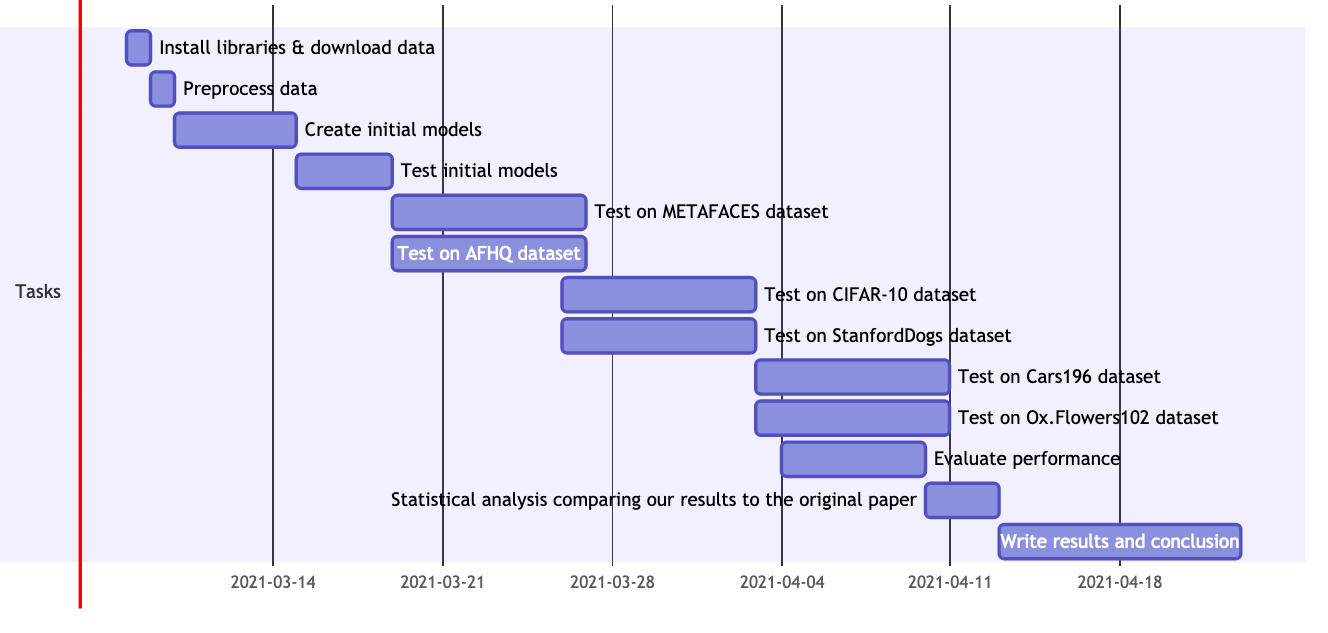
\includegraphics[width=1\textwidth]{figs/timeline.png}
    \caption{Project Timeline}
\end{figure}

\end{itemize}



\section{Conclusions}

%Sum up, including your opinion on each approach.  Also, list any questions that you have for the instructor and TA regarding your project work.
GAN approach is an efficient generative modeling approach, but its high demand for dataset size limits small-sized datasets applications. The experiments in Keras et al. proposed ADA as a method to increase the GAN approach's feasibility for small-size datasets. By applying an adaptive discriminator augmentation mechanism, the GAN approach can generate good results with small datasets. In our project, we will attempt to reproduce similar results to the models' performance reported in the paper, following the source code and the methodology reported in the paper, we will test ADA on three datasets from the original paper and three additional new datasets. As described above, after the preprocessing of data, we will follow the pipeline where the baseline is StyleGAN2. The paper provides good details of the methodology and well-documented source code that will allow us to test whether we can reproduce the results.


%\textcolor{red}{Remember to cite sources using BibTeX and add those references to the end of this document!}

%It is okay to cite some websites and tutorials (if you first look up how to cite them properly!), but you must also cite some refereed publications from conferences and journals.




%%%%%%%%%%%%%%%%%%%%%%%%%%%%%%%%%%%%%%%%%%%%%%%%%%%%%%%%%%%%%%%%%%%%%%%%%%%%%%%%%%%%%%%%%%%%%%%%%%%%%%%%%%%%%%%%%%%%%%%%%%%%%%%%%%%%%%%%%%%%%%%%%%%%%%%%%%%%%%%%%%%%%%%%%%%%%%%%%%%%%%%%%%%%%%%%%%%%%%%%%%%%%%%%%%%%%%%%%%%%%%%%%%%%%%%%%%%%%%%%%%%%%%%%%%%%%%%%%%%%%%%%%%%%%%%%%%%%%%%%%%%%%%%%%%%%%%%%%%%%%%%%%%%%%%%%%%%%%%%%%%%%%%%%%%%%




%%%%%%%%%%%%%%%%%%%%%%%%%%%%%%%%%%%%%%%%%%%%%%%%
%%%%%%%%%%%%%%%%%% MILESTONE 3 %%%%%%%%%%%%%%%%%%
%%%%%%%%%%%%%%%%%%%%%%%%%%%%%%%%%%%%%%%%%%%%%%%%

\chapter{Milestone 3: Progress Report 1}

\section{Introduction}
\label{sec:M3-intro}

% Remind the reader of the problem you're working on and what your approach is.  Briefly summarize what your results are so far.
% Also, remember to update your abstract when you've completed this chapter.

As described in the previous chapters, our project aims to evaluate the ADA mechanism's reproducibility and replicability in training GAN with limited data. 

Generative Adversarial Networks (GAN) is a generative modeling approach using deep learning techniques to automatically discover and learn the input patterns to generate an output that would plausibly appear as if it was sampled from the original dataset\cite{goodfellow2014generative}. The structure constructed in GAN has a generator model and discriminator model connected, allowing the superficially plausible data generated by the generator to proceed to the discriminator model to do discrimination with the real data and penalize the generator if there’s an implausible result detected \cite{creswell2018generative}. The built-in structure makes GAN approach powerful to generate a sample; however, GAN's strong power cannot be performed appropriately for the limited dataset problems. When the GAN approach is applied on limited datasets, the discriminator will overfit to training data examples, and the training eventually diverges. Furthermore, when the augmentation of the dataset is introduced to resolve the overfitting, the augmented distribution can be induced, which is undesirable for sample generation\cite{zhao2020improved}. To eliminate the obstruction of the overfitting problem in a limited dataset for the GAN approach, the research by Kerras et al. came up with one method to do this by applying a wide variety of augmentation methods\cite{karras2020training}. \\
Our project is to provide a complete evaluation of the proposed generative image training models by Kerras et al. We are following the method and code provided in the paper, using the StyleGAN2-ADA architecture to assess its reproducibility and ability to classify datasets with limited data. The datasets we are using in this project include METFACES\cite{karras2020training}, AFHQ (WILD, DOG, CAT)\cite{choi2020stargan}, CIFAR-10\cite{krizhevsky2009learning}, StandfordDogs\cite{KhoslaYaoJayadevaprakashFeiFei_FGVC2011, imagenet_cvpr09}, Cars196\cite{KrauseStarkDengFei-Fei_3DRR2013}, and OxfordFlowers102\cite{Nilsback08}. We have preprocessed the images of all these datasets and trained three datasets for at least one day. Here, we report results from these three datasets:
\begin{enumerate}
\item METFACES
\item AFHQ-WILD
\item OxfordFlowers102
\end{enumerate}

We used the results that we have so far to calculate and report the Frechet Inception Distance (FID) alongside the hyperparameters that were used in each dataset. We found that we're able to reproduce two datasets presented in the original paper – METFACES and AFHQ-WILD. We also found that the model can produce good results from the new dataset (i.e., datasets that were not tested in the original paper) based on our results from the OxfordFlowers102 dataset. We report and discuss these results about the adaptive discriminator augmentation (ADA) mechanism. 


%\begin{enumerate}
%\item Metfaces: 20.0700
%\item AFHQ-WILD: 2.3100
%\item AFHQ-CAT: 151.2348
%\item AFHQ-DOG: 11.3855
%\item StanfordDogs: 33.0543
%\item Cars196: 11.9445
%\item OxfordFlowers102: 8.1900
%\end{enumerate}

\section{Experimental Setup}
\label{sec:M3-setup}

%Describe the setup of your experiments so far in sufficient detail for the reader to reproduce them.  Include data sources, preprocessing used, architectures/other approaches used, hyperparameter values used, performance measures used, other relevant items (e.g., cross-validation).

\begin{itemize}
\item\textbf{Environment setup}. This project creates an Anaconda3 environment to install required packages and dependencies to compile and train the StyleGAN2-ADA architecture. Specifically, we loaded GCC 6.1 and built a GPU-capable TensorFlow 1.14 environment with Python 3.7, Numpy 1.14.3, CUDA 10.0 toolkit, and cuDNN 7.5.

\item \textbf{Data sources}. In this project, we use multiple datasets to test the StyleGAN2-ADA architecture proposed by Karras et al. The datasets we report here are the ones we sufficiently trained using the StyleGAN2-ADA architecture, and these datasets are: 
 \begin{enumerate}
 \item \textit{Metfaces}, which consists of 1336 high-quality faces extracted from the collection of Metropolitan Museum of Art with ($1024 \times 1024$) resolution. 
 \item \textit{AFHQ-Wild}, which consists of 4738 images of wildlife animals, with ($512 \times 512$) resolution.
  \item \textit{OxfordFlowers102}, which consists of 8189 images of flowers commonly occurring in the United Kingdom in various image resolutions.
   \end{enumerate}

\item \textbf{Preprocessing}. 
\begin{itemize}

\item \textit{\textbf{Resizing}.} We resize our dataset to half the original size that was used in the paper, that is, a resized resolution of ($256 \times 256$) for all datasets except for the METFACES dataset, which we resized to ($512 \times 512$). We have decided to resize the images to a smaller size due to the GPUs resources' limitation and overall computing power compared to the original paper.

\item \textbf{\textit{Dataset Augmentation}}. The augmentation itself is considered a part of the preprocessing task. However, we decide to dedicate a subsection because it is the core of the original paper. In this project, we follow the same augmentations proposed by Karras et al. in the original paper. These augmentations consist of 18 transformations: geometric (7), color (5), filtering (4), and corruption (2). Figure 3.1 shows a visual demonstration of each transformation effect.

 \begin{enumerate}
 \item \textbf{Geometric and color transformations.}\\ 
 \begin{enumerate}
 \item \textit{\textbf{Pixel blitting.}}
 We begin by using pixel blitting to copy existing pixels as-is without blending between adjacent pixels. This process consists of x-flips, 90 degrees rotations, and integer translations. This produces a $3\times3$ matrix. Moreover, each transformation with probability (\textit{p}) by sampling its parameters from uniform distribution (5th, 35th, 65th, 95th) percentiles.
  \item \textit{\textbf{General geometric transformations.}}
  This process consists of isotropic scaling, arbitrary rotation, anisotropic scaling, and fractional translation. Here, rotations are applied less frequently (at least one rotation is equal (\textit{p})). Afterward, we use a low pass filter to ensure that interpolating at the original resolution filters out frequencies above Nyquist. 
\item \textit{\textbf{Color Transformation.}}
This process consists of adjusting brightness, contrast, and saturation. Moreover, it consists of flipping the luma axis while keeping the chroma unchanged and rotating the hue axis by an arbitrary amount.\\
  \end{enumerate}
  
  \item \textbf{Image-space filtering and corruptions.} \\
  \begin{enumerate}
  \item \textbf{\textit{Image-space filtering.}}
  this process turns the content of the images to 4 non-overlapping band through 4 transformations.  Afterwards, we perform filtering using amplifying filters. Then, we add separable convulsions for images using reflection padding. 
  \item \textbf{\textit{Image-space corruptions.}}
  image corruptions is introduced by applying RGB noise and cutouts. The is introduced in using its standard deviation from half of the normal distribution. Cutout are performed by setting pixels to zero within a rectangular area of a predefined size depending on the image dimension.
  \end{enumerate}
   \end{enumerate}

\begin{figure}[!h]
  \centering
  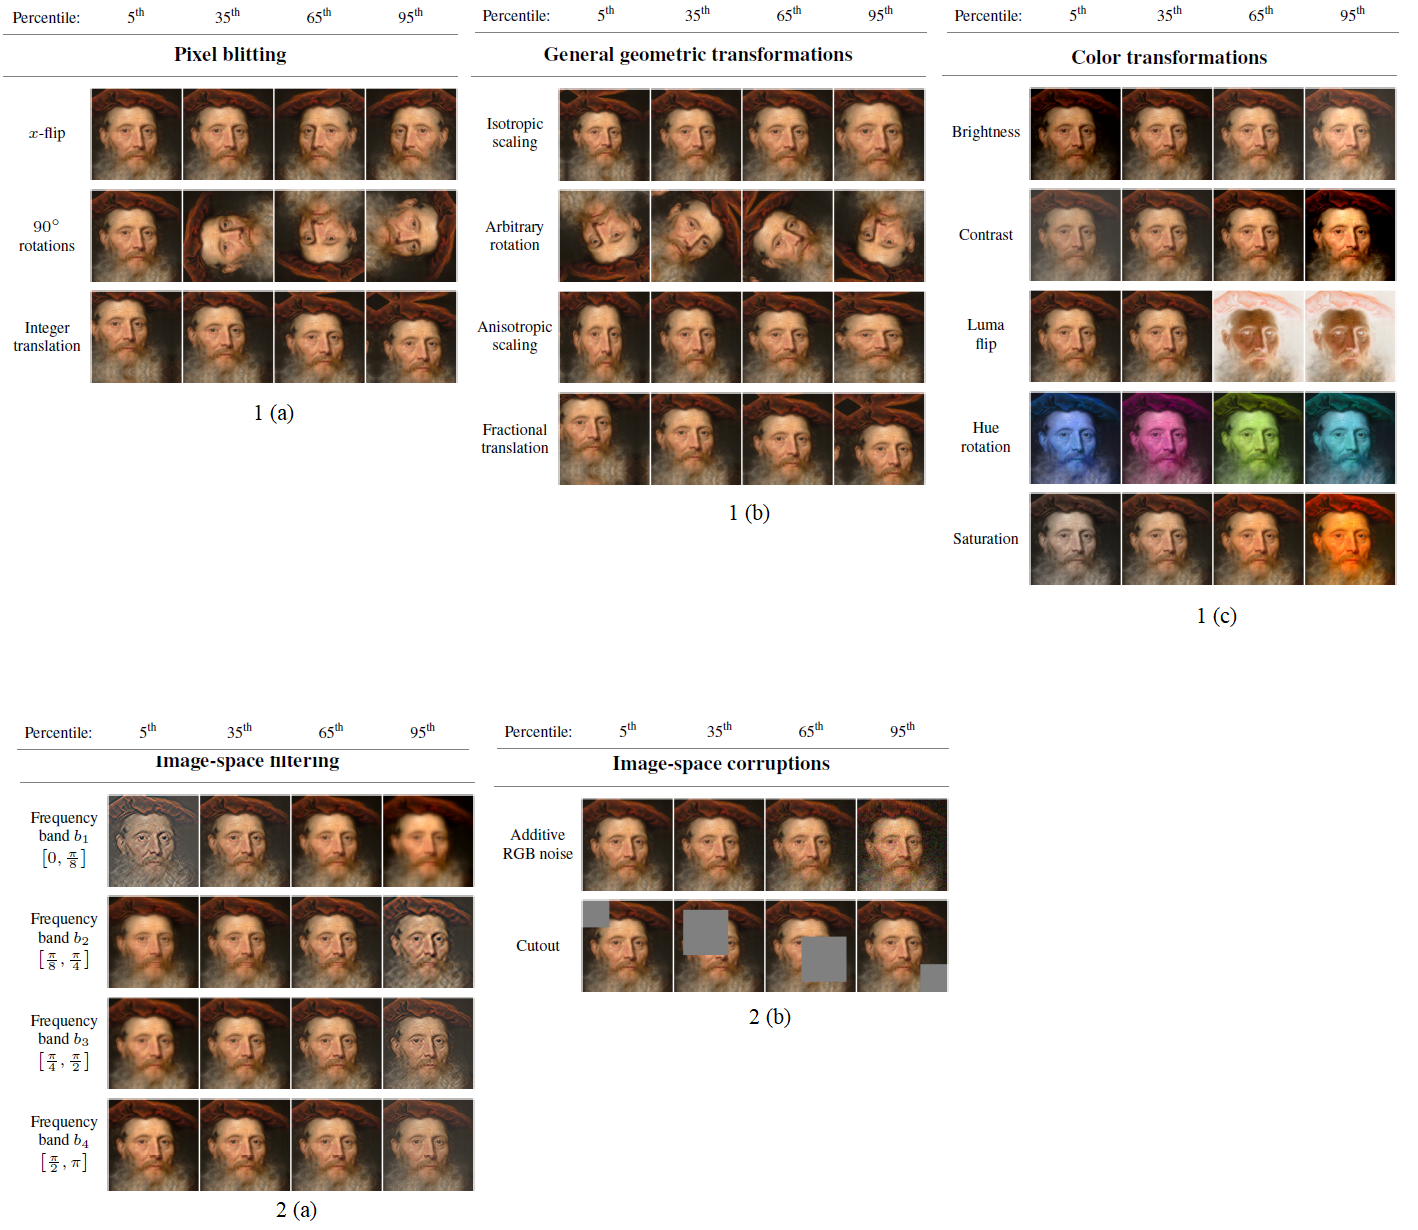
\includegraphics[width=\linewidth]{figs/aug.png}
\caption{Visual Sample demonstrating different augmentations proposed by Karras et al. and used by the ADA mechanism.}
\end{figure}

\end{itemize}

\item \textbf{Hyperparameters.} The hyperparameters that we used to train our models are described in Table 3.1.

\begin{table}[!ht]
\caption{Hyperparameters used in each experiment.}
\centering 
\begin{tabular}{ |p{4cm}|p{1.8cm}|p{2.3cm}|p{2.9cm}| }
 \hline
 Parameter & Metfaces & AFHQ-WILD  & OxfordFlowers102\\
 \hline
 Resolution             & $512\times 512$   & $256\times 256$     & $256\times 256$\\
 No. of GPUs (Tesla V100)         & 2        & 2          & 2\\
 Base feature maps           & 16384    & 8192    & 8192\\
 Training time (hrs)  & 22.42    & 35.14      & 20.71\\
 Minibatch size         & 16       & 32         & 32\\
 Minibatch stddev       & 4        & 4         & 4\\
 Learning rate       & 0.0025      & 0.0025        & 0.0025\\
 R1 regularization      & 3.2768   & 0.4096     & 0.4096\\
 Dataset x-flips        & Yes      & Yes        & Yes\\
 Mixed-precision        & Yes      & Yes        & Yes\\
 Mapping net depth      & Yes      & Yes        & Yes\\
 Style mixing reg.      & Yes      & Yes        & Yes\\
 Path length reg.       & Yes      & Yes        & Yes\\
 Resnet D               & Yes      & Yes        & Yes\\
 \hline
\end{tabular}
\end{table}

\item \textbf{Performance measure.}\\
To test our model performance, we use FID as a function of training set size and compare our results against the original paper's FID scores.


\end{itemize}


\section{Experimental Results}
\label{sec:M3-results}
%Present your results so far using tables, figures, confusion matrices, etc.\ (whatever is appropriate). 

In this section, we provide results of training multiple small datasets using the StyleGAN2-ADA architecture as proposed by Karras et al. Table 3.2 shows details about training time, our model's FID score per dataset, and the original paper's FID scores. 


\begin{table}[!ht]
\caption{Fréchet inception distance (FID) results}
\centering 
\begin{tabular}{ |p{3cm}|p{3cm}|p{1.5cm}|p{3cm}| }
 \hline
 Dataset & Training time (hrs) & Our FID & Original paper FID\\
 \hline
 METFACES        & 22.42    & 20.07 & 18.22\\
 AFHQ-WILD       & 35.14    & 2.31 & 3.05\\
 OxfordFlowers102& 20.71    & 8.19 & NA (new dataset)\\
 \hline
\end{tabular}
\end{table}
In Figure 3.2 to Figure 3.4, we are showing the comparison between the output images and the real ones, where (a) part representing real images, and (b) part representing the fake images reported at this point. The high similarity between fake and real images and the good FID are supporting each other.



\section{Discussion}

%Discuss your experimental results, drawing conclusions that are supported by your experimental results of Section~\ref{sec:M3-results}.  Be careful not to draw conclusions that are not supported by the evidence you present! Discuss how these results will influence your future experiments.

In Section 3.3, we provide the results we have until now. Training METFACES dataset took around 22 hours after that; we reached an FID of 20. The original paper FID is 18.22 showing that the authors' implementation of the architecture is reproducible. Moreover, it indicates that StyleGAN2-ADA provides a significant improvement over the baseline algorithm StyleGAN2 because our implementation of the model already beats the StyleGAN2 accuracy reported in the original paper.\\
The two datasets tested in the original paper, METFACES and AFHQ-WILD, returned comparable FID scores to what is reported in the paper in a shorter time.  We believe that although resizing the images decreased the output quality, it did noticeably speed up the training time required to reach reasonably good results in the two datasets with FID scores of 20.07 and 2.32, respectively. We also demonstrate that we could achieve an FID score of 8.19 after training the Oxford-flowers dataset for about 29 hours.

\section{Conclusion}

%Sum up, including a summary of your results so far (recapitulating that from Section~\ref{sec:M3-intro}).  Also, describe your plans for future work and list any questions you have for the instructor and TA regarding your project work.
We demonstrated that we could reproduce FID scores with the METFACES and AFHQ-WILD datasets comparable to the original paper's results and good FID scores with a new OxfordFlowers102 dataset. In the next report, we will test if the results from StyleGAN2-ADA against results generated with StyleGAN2 and use the appropriate statistical test to demonstrate whether StyleGAN2-ADA is significantly better (i.e., returns better FID scores) than StyleGAN2. Then, we will attempt to reproduce results from the other two AFHQ datasets and CIFAR-10, this time without resizing the images. We will also further test the replicability of the model using additional datasets, including StanfordDogs and Cars196. Overall, in the next report, we will include results from datasets without image resizing and different sets of hyperparameters, results from StyleGAN2 to statistically compare it against StyleGAN2-ADA, and results from new datasets to evaluate the model's replicability.

% Aiming to reproduce similar results to the performance reported in the paper, we are following the source code reported in the paper to apply ADA on six small datasets, where three from the original paper and another three are new. Based on the situation we are in, some tiny changes also were introduced compared to the paper: to adapt to the GPU we have, we decreased the size of the images in datasets. For now, we have finished the preprocessing of datasets, and sent them to the StyleGAN2-ADA architecture, starting the training. Therefore, in the next milestone, we will provide training results of other datasets including AFHQ-CAT, AFHQ-DOG, and StanfordDogs. 


\begin{figure}[!t]%
    \centering
    \subfloat[\centering Real images]{{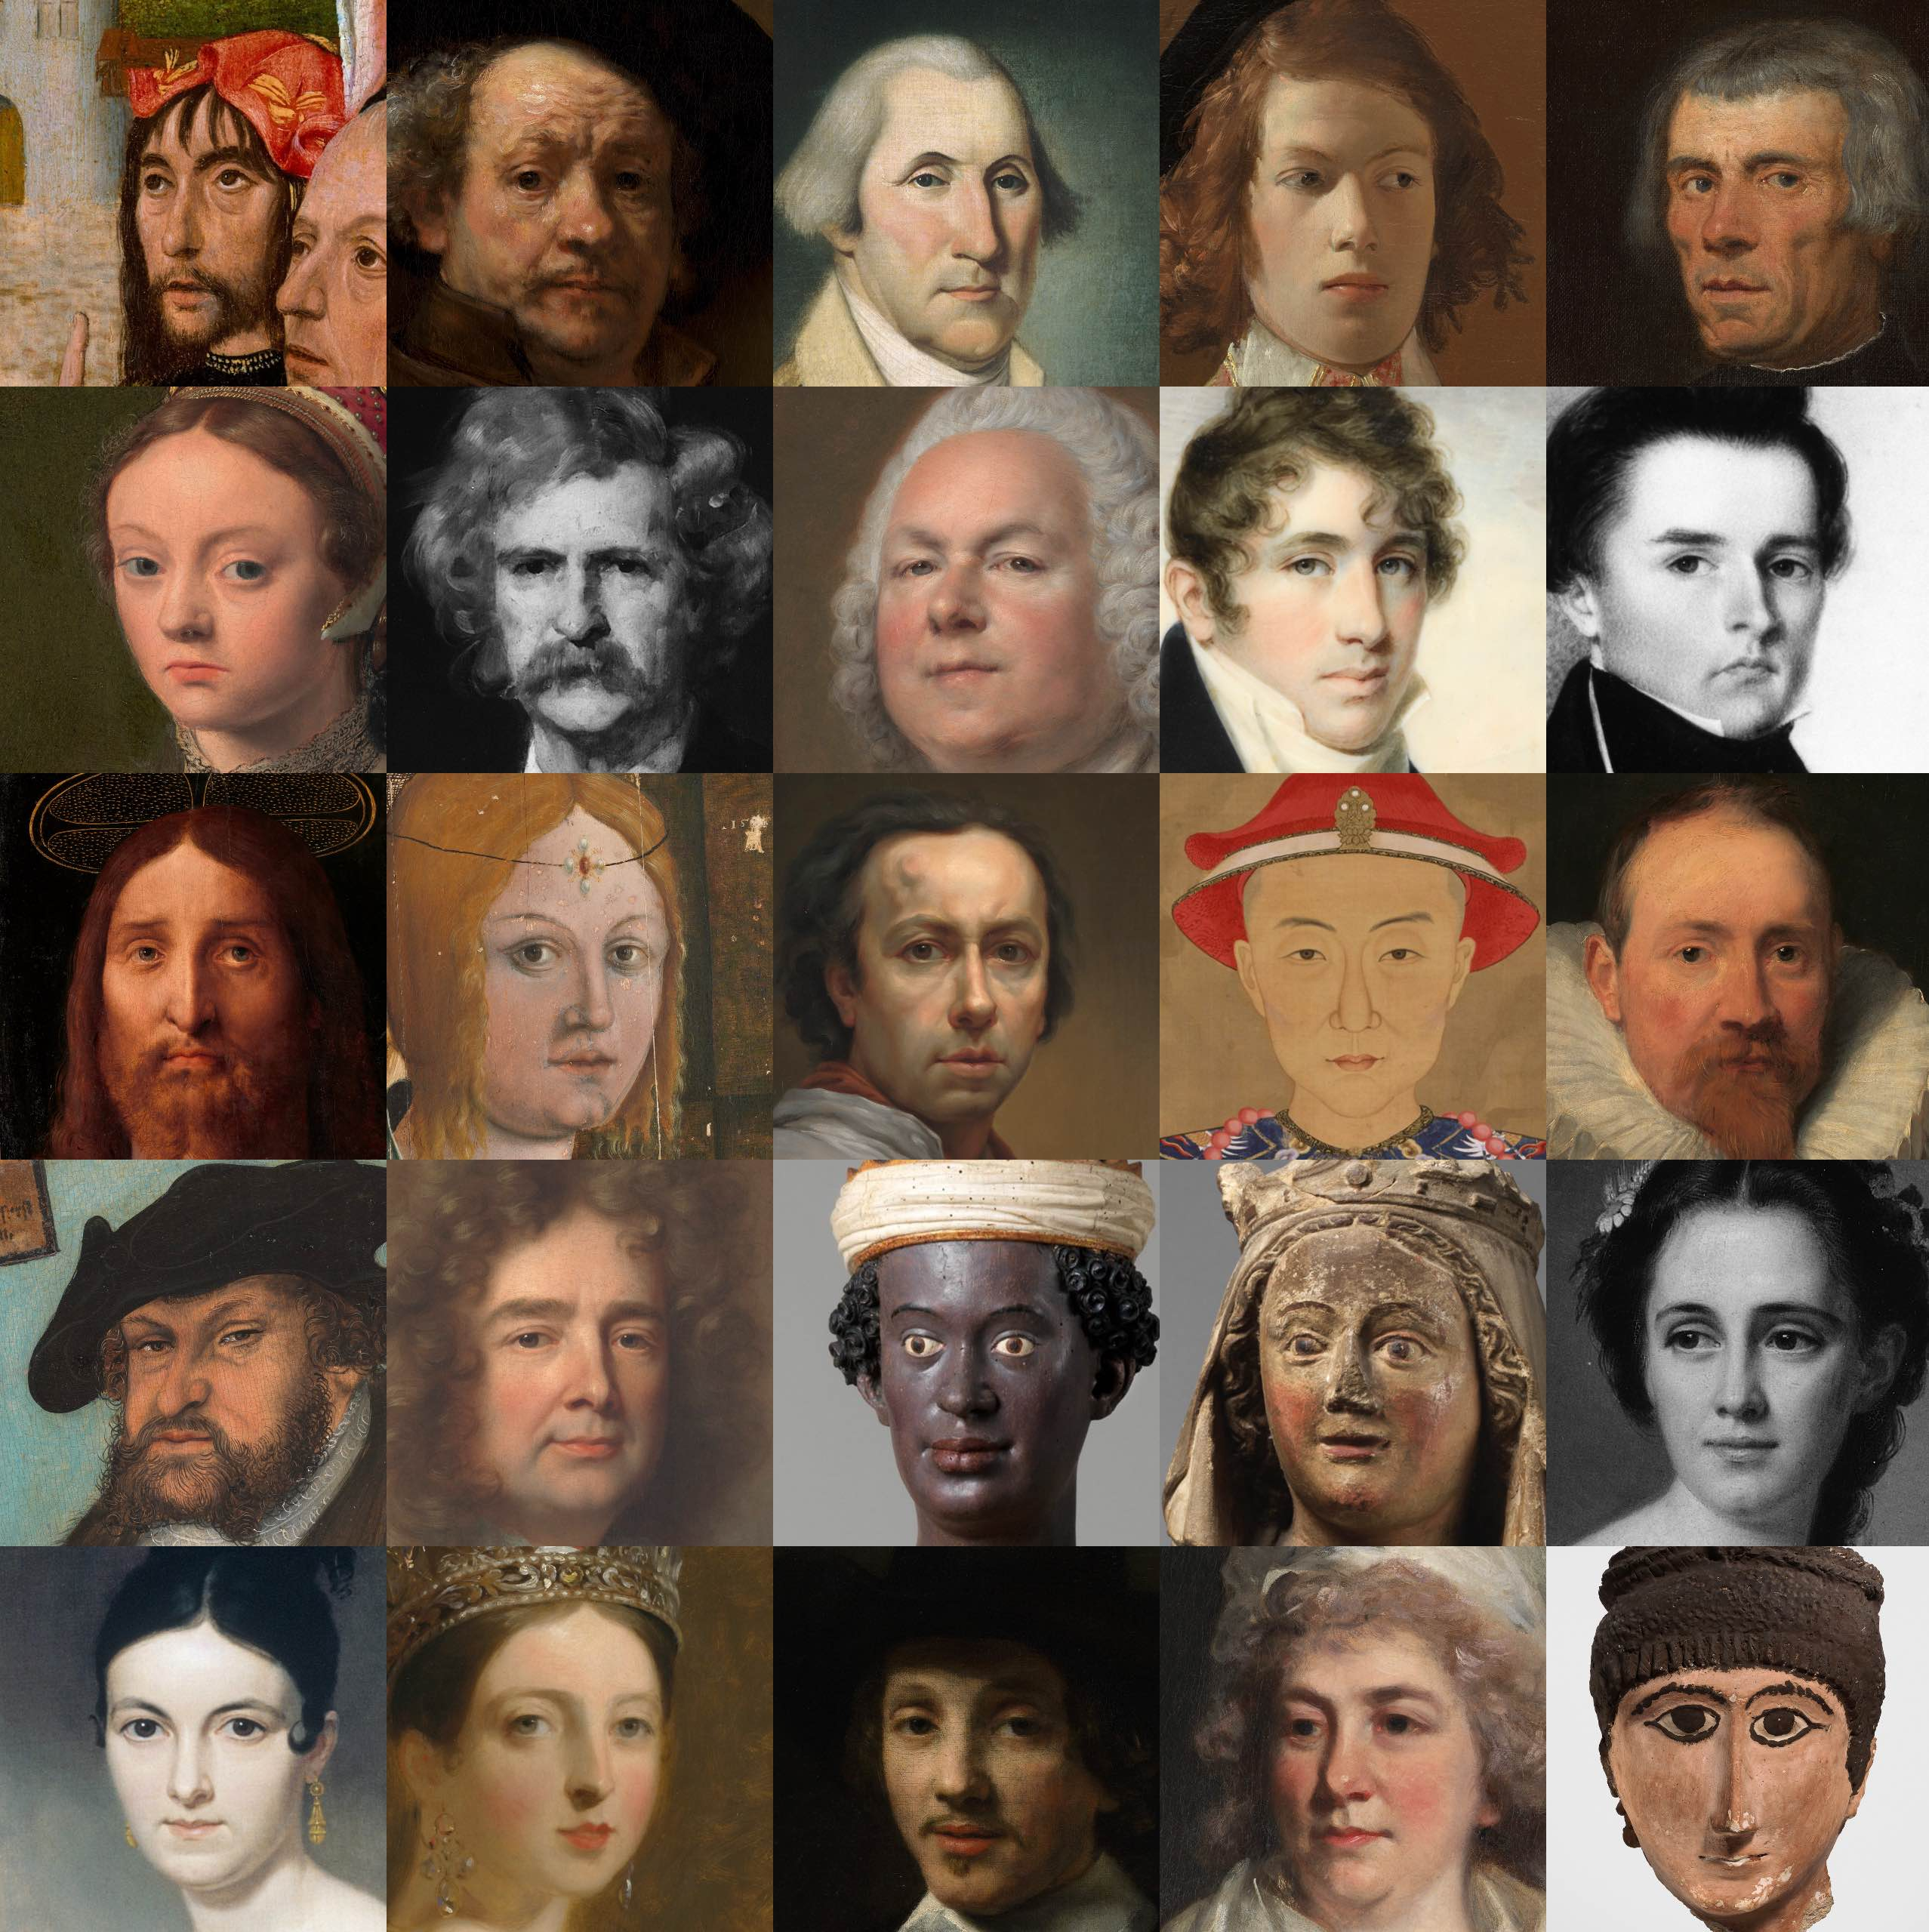
\includegraphics[width=8.5cm]{figs/reals_metfaces.jpg} }}
    \quad
    \subfloat[\centering Fake images]{{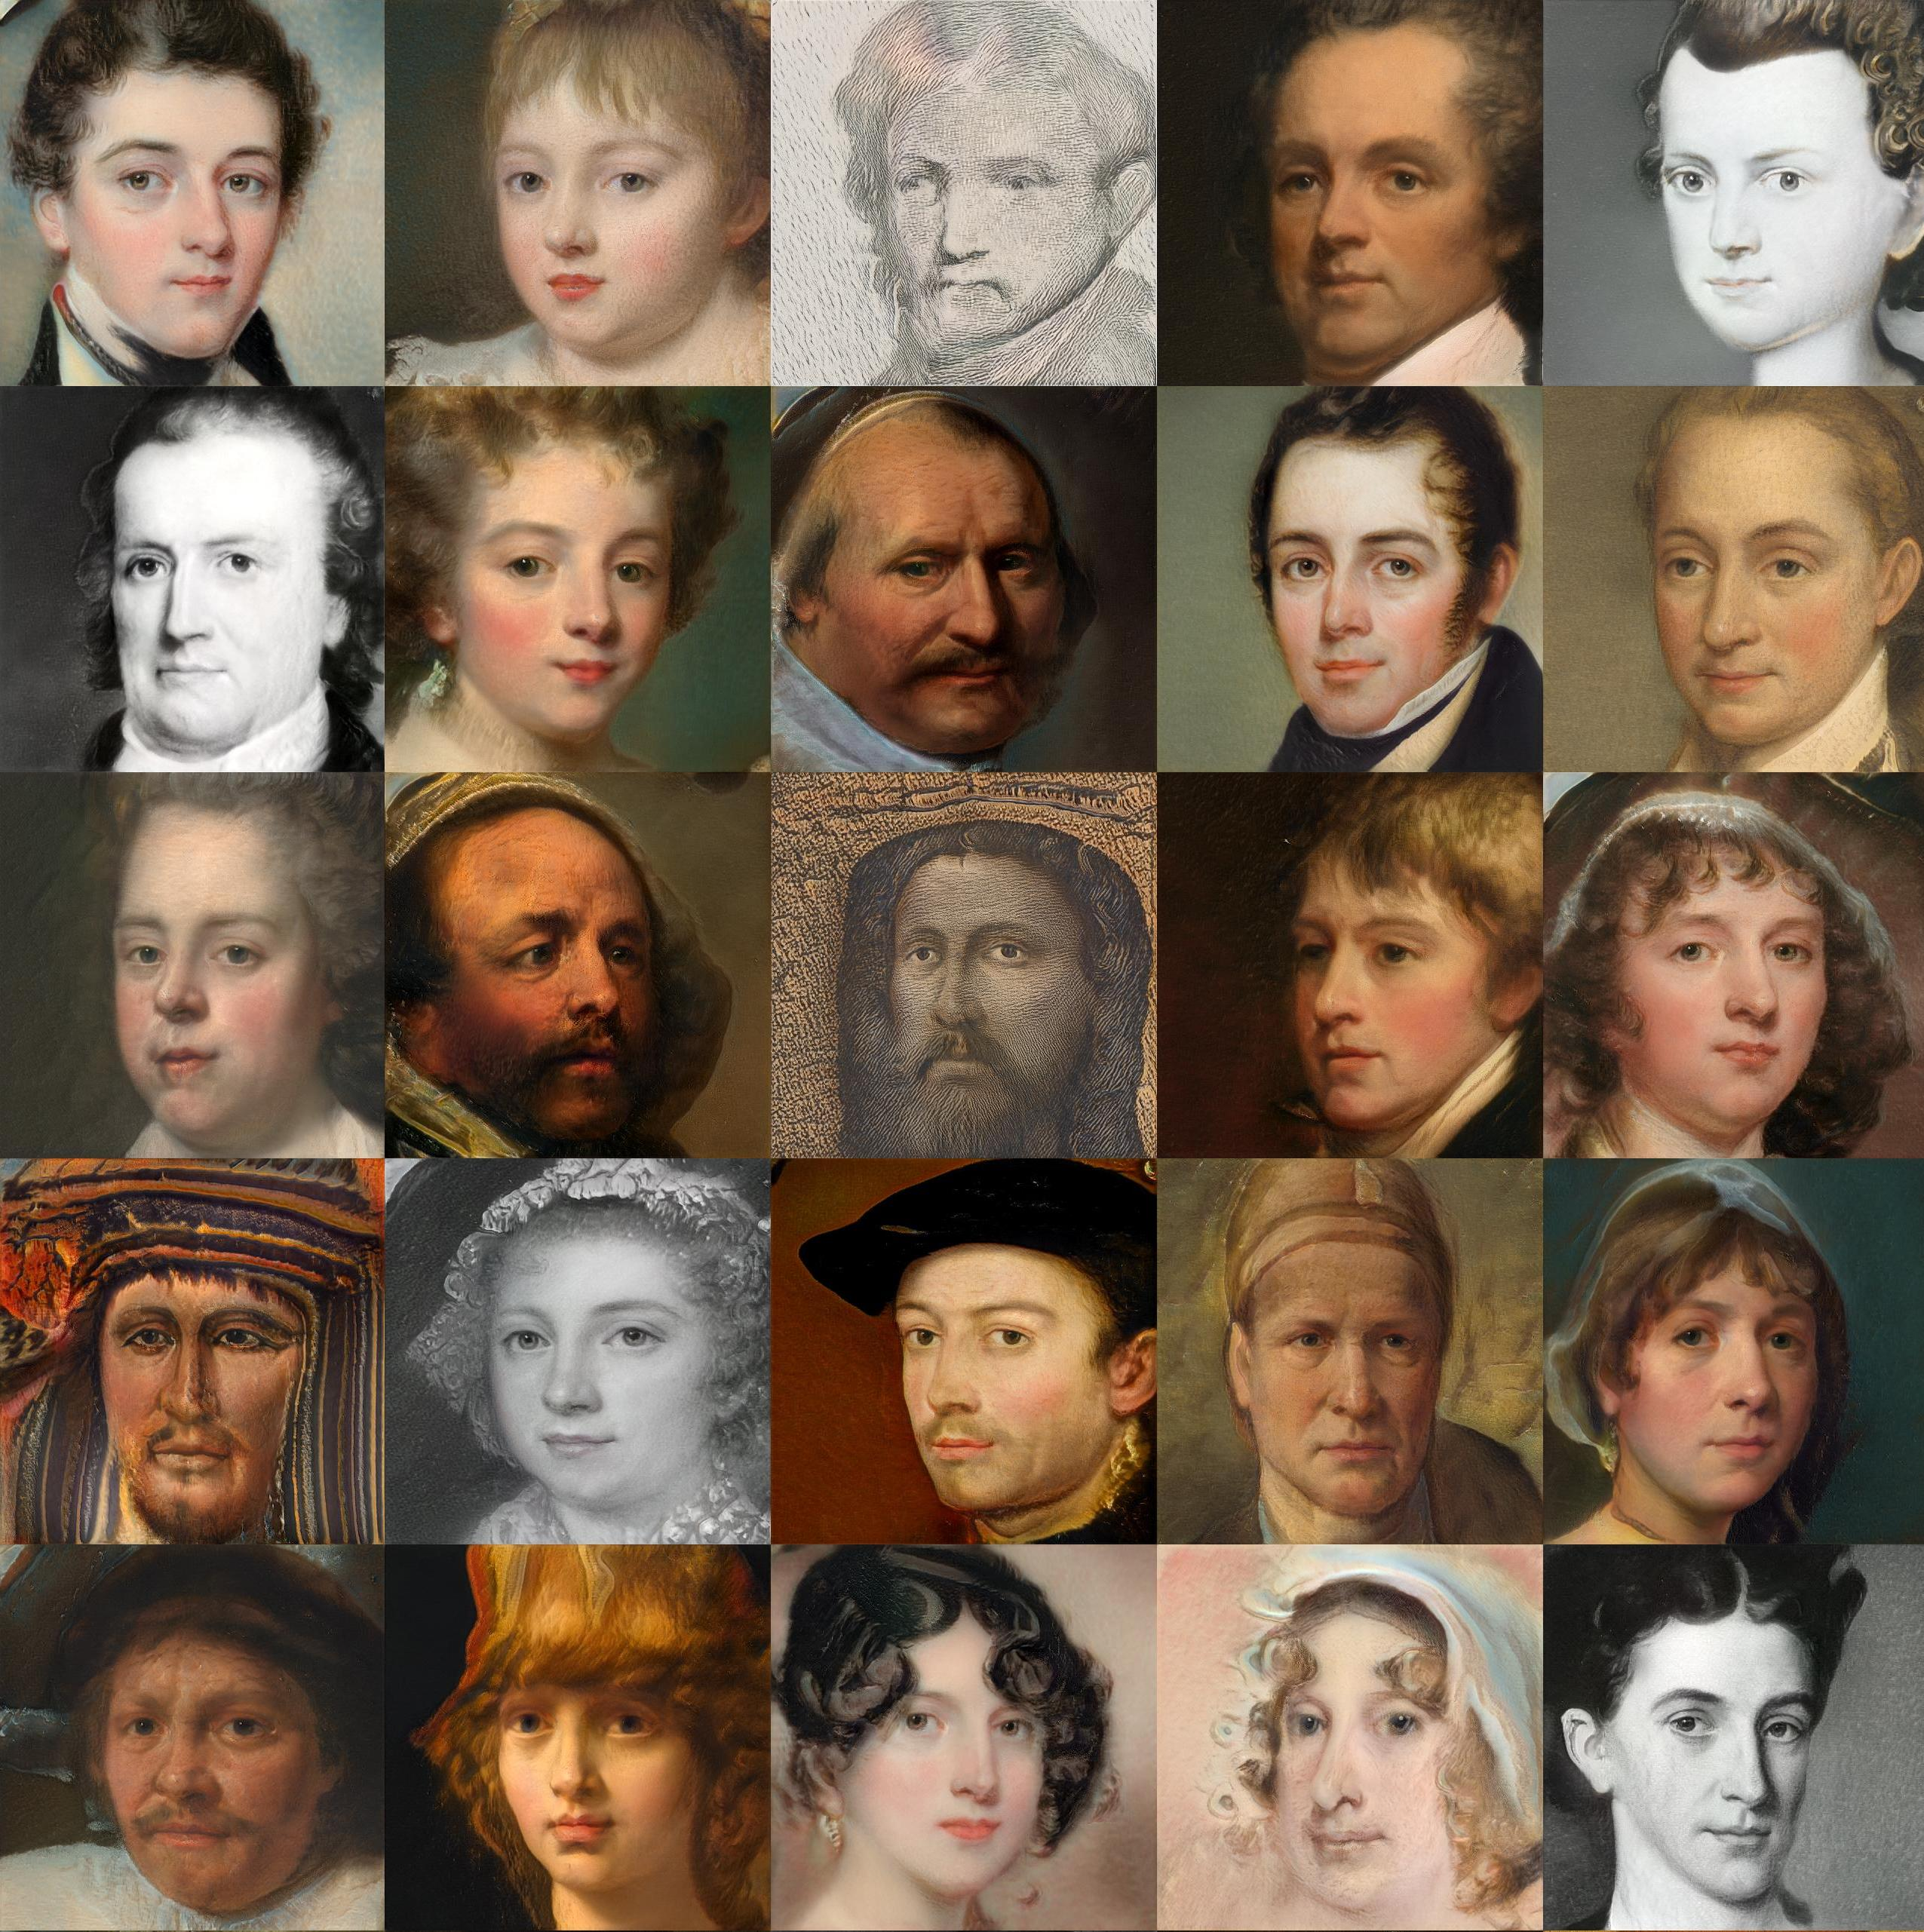
\includegraphics[width=8.5cm]{figs/fakes_metfaces.jpg} }}%
    \caption{Snapshots of METFACES real and fake images.}%
    \label{fig:example}%
\end{figure}

\begin{figure}[!t]%
    \centering
    \subfloat[\centering Real images]{{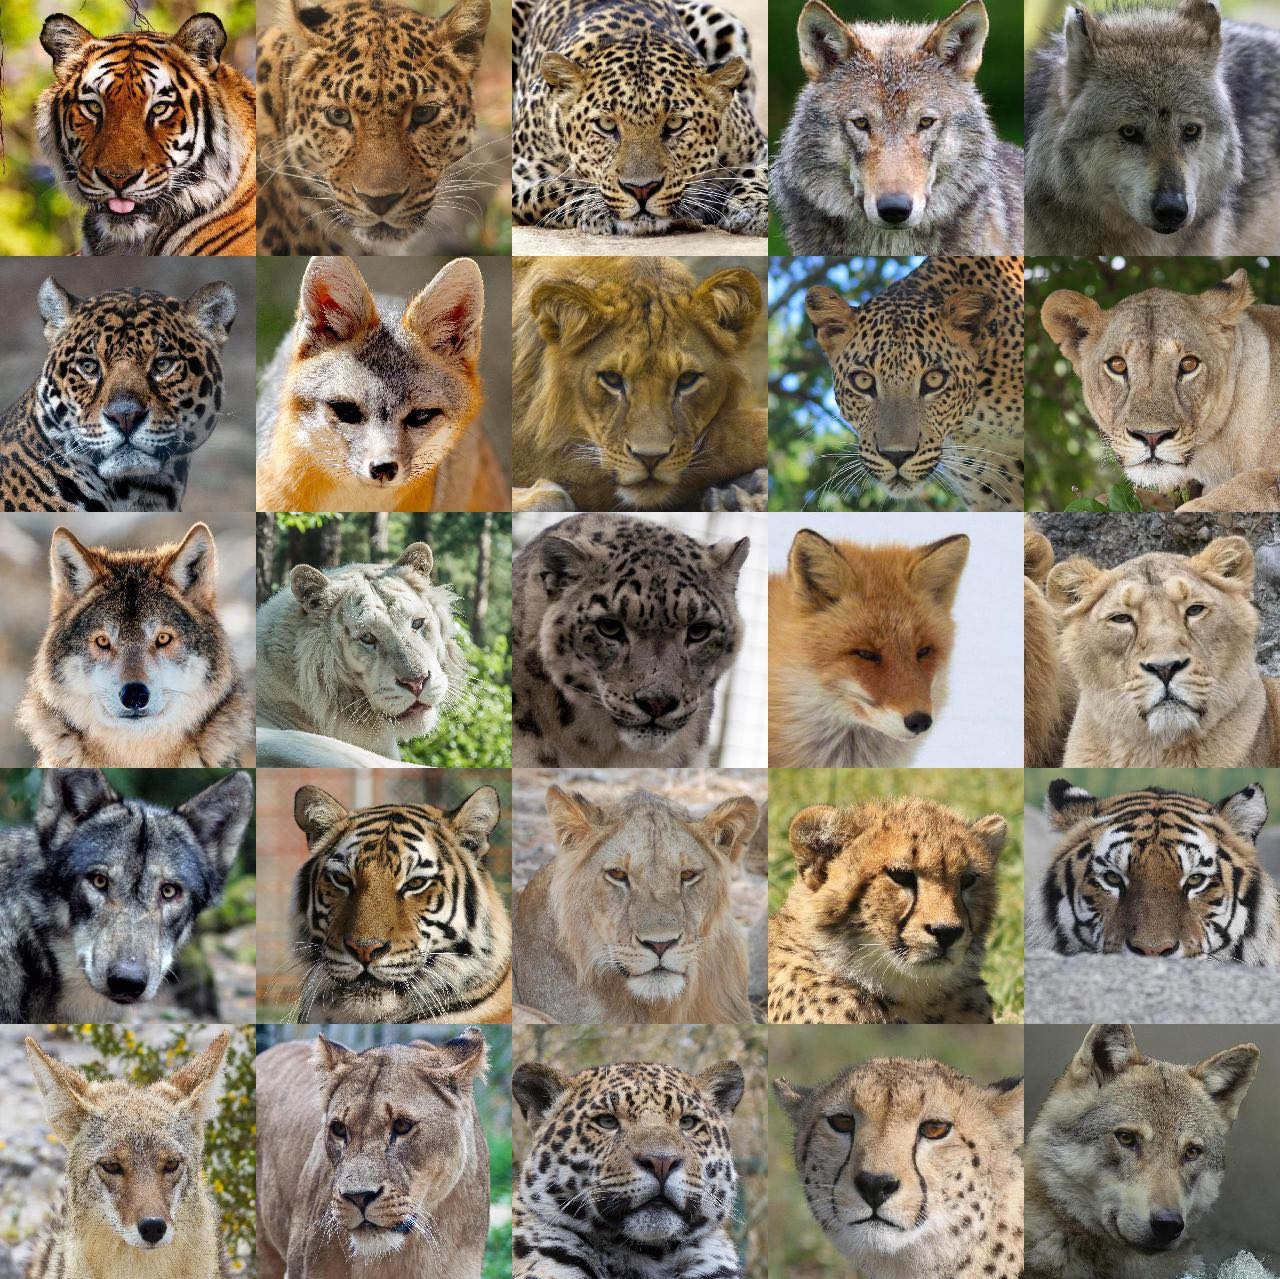
\includegraphics[width=8.5cm]{figs/reals_wild.jpg} }}
    \quad
    \subfloat[\centering Fake images]{{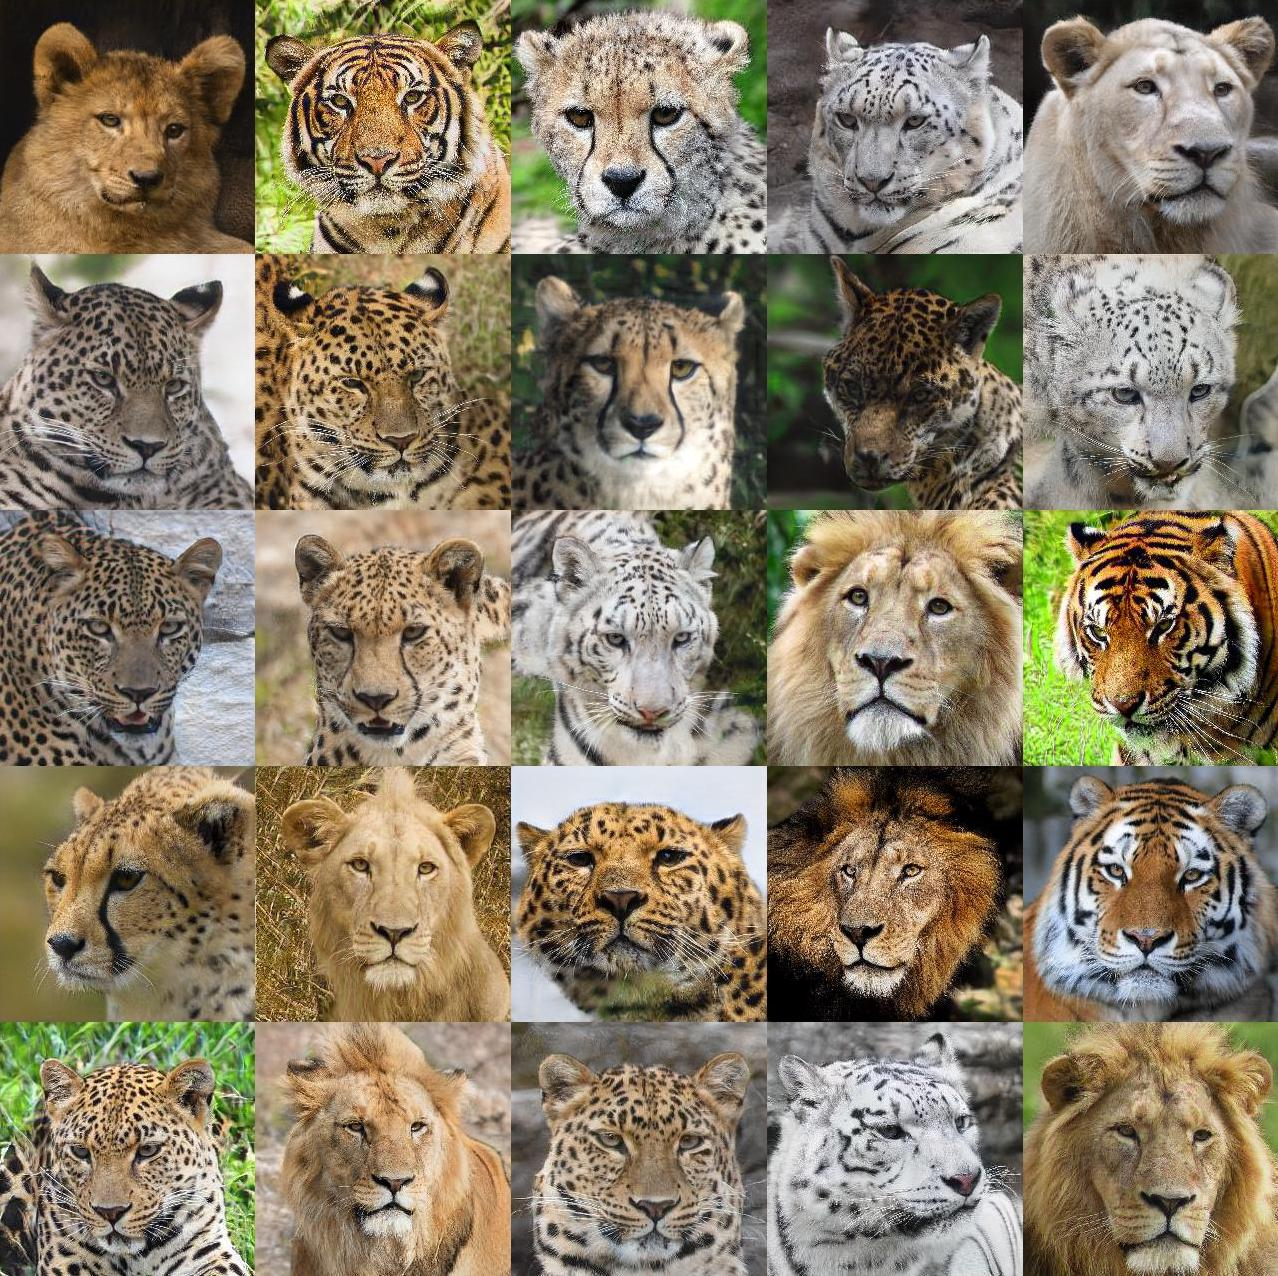
\includegraphics[width=8.5cm]{figs/fakes_wild.jpg} }}%
    \caption{Snapshots of AFHQ-WILD real and fake images.}%
    \label{fig:example}%
\end{figure}

\begin{figure}[!t]%
    \centering
    \subfloat[\centering Real images]{{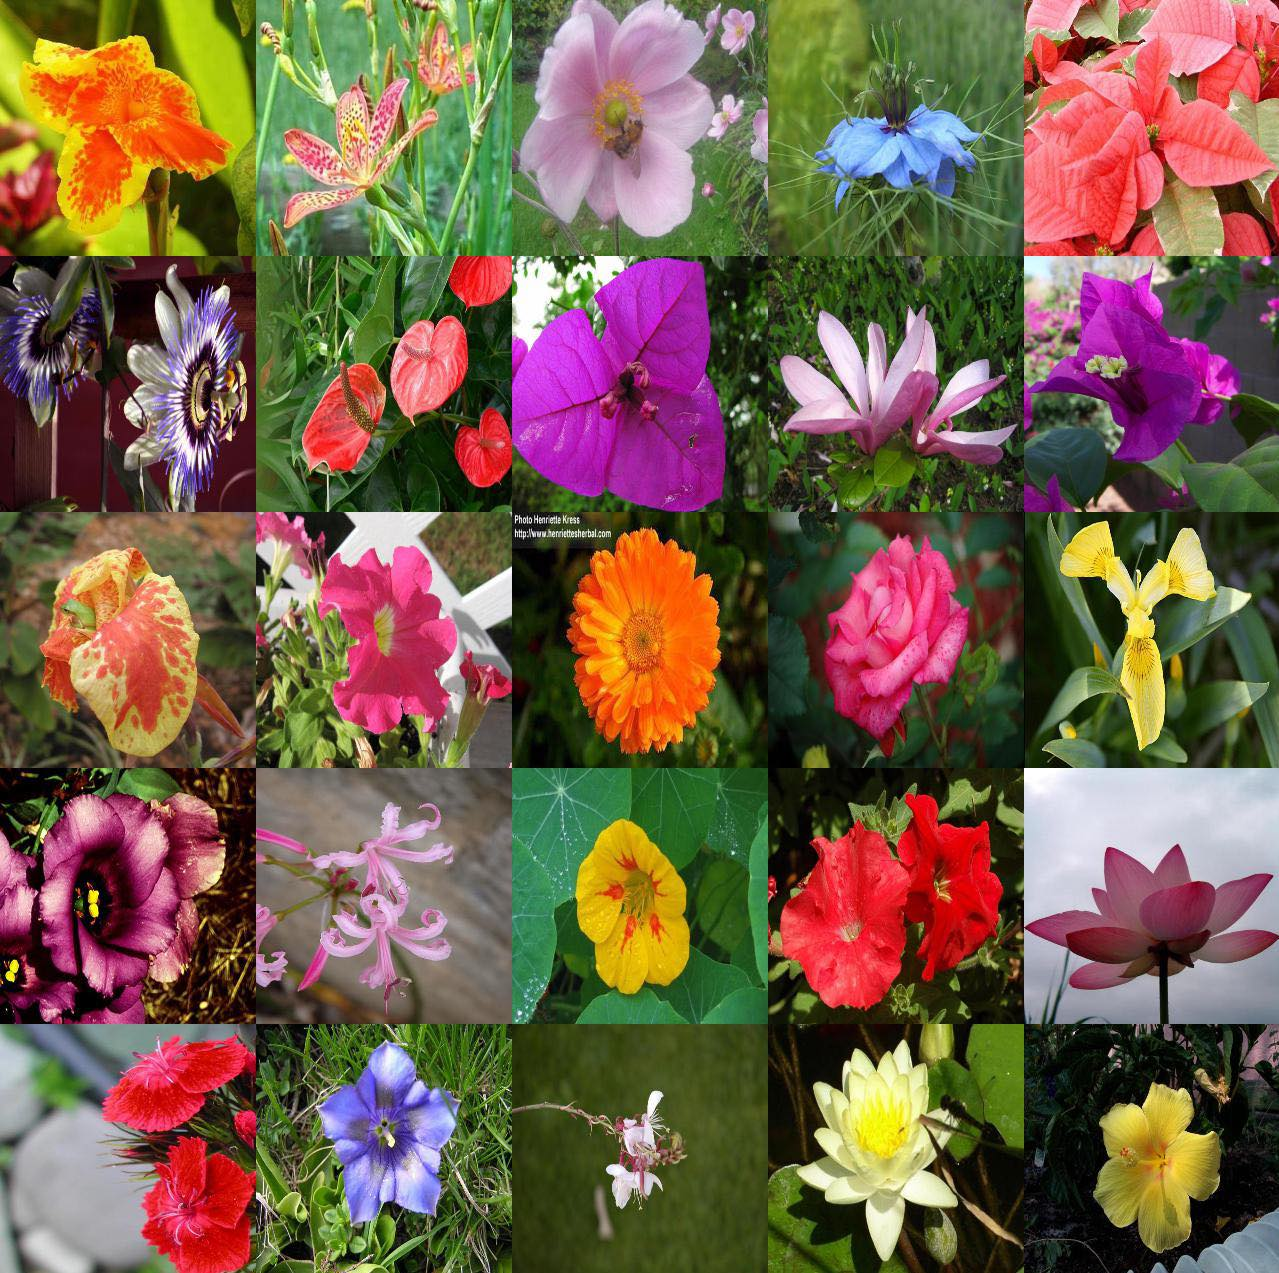
\includegraphics[width=8.5cm]{figs/reals_flowers.jpg} }}
    \quad
    \subfloat[\centering Fake images]{{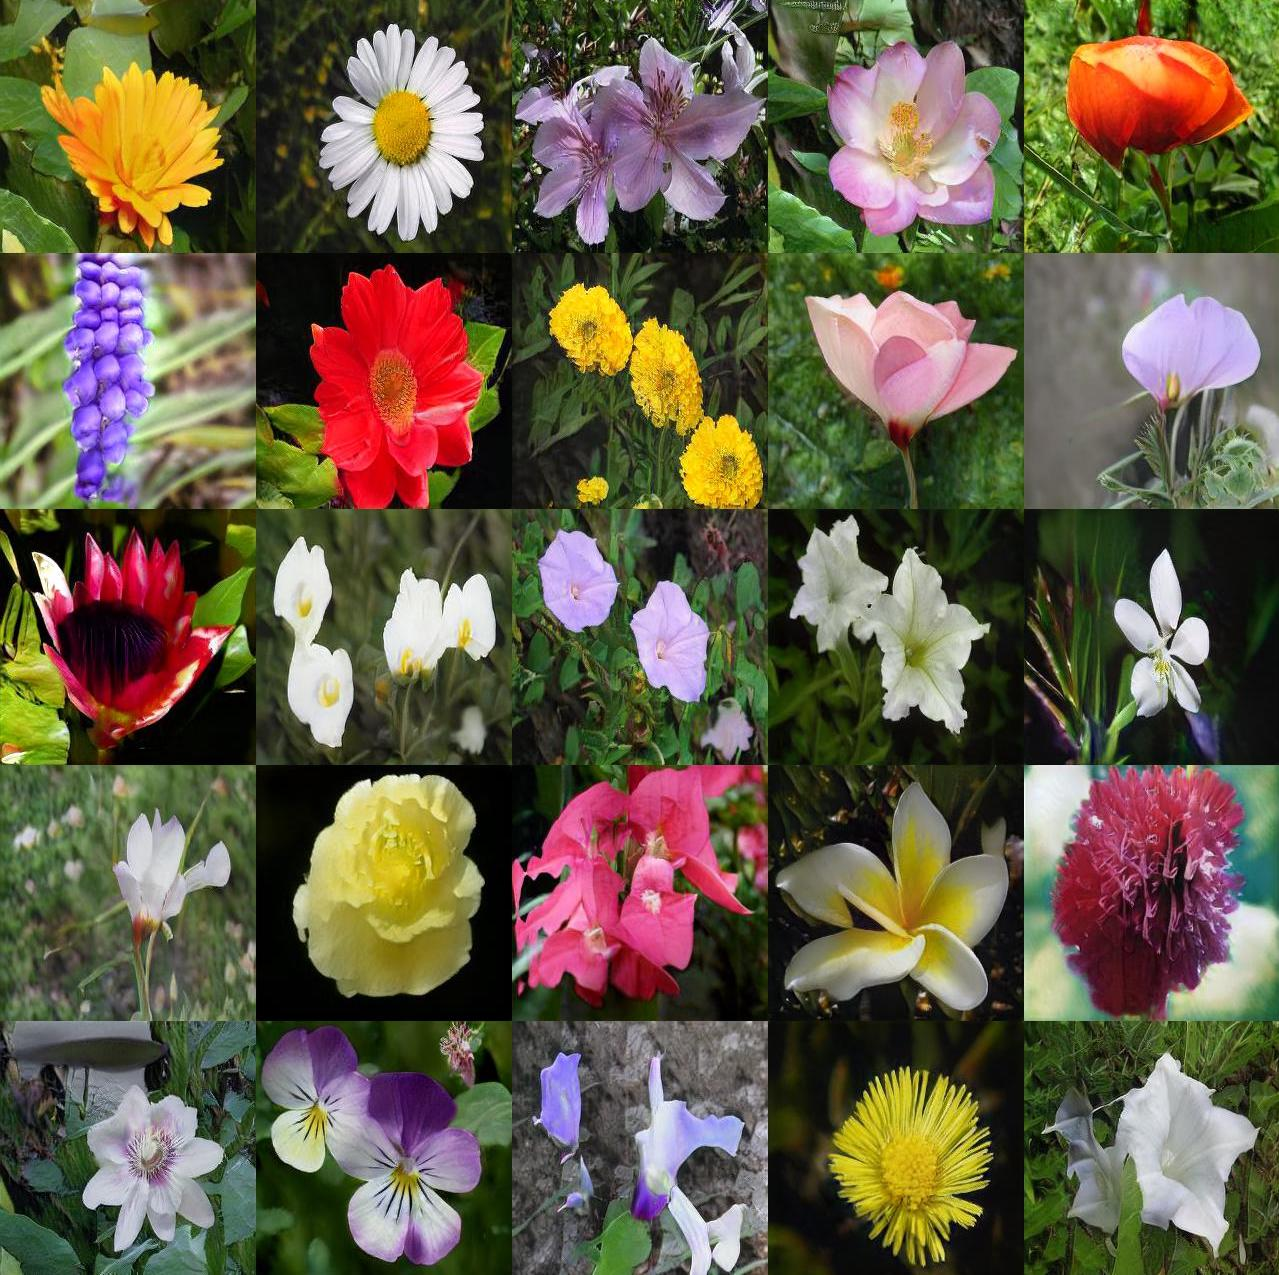
\includegraphics[width=8.5cm]{figs/fakes_flowers.jpg} }}%
    \caption{Snapshots of OxfordFlowers102 real and fake images.}%
    \label{fig:example}%
\end{figure}



%\textcolor{red}{Remember to cite sources using BibTeX and add those references to the end of this document!}

%It is okay to cite some websites and tutorials (if you first look up how to properly cite them!), but you must also cite some refereed publications from conferences and/or journals.


\bibliographystyle{plainurl}
\bibliography{main}

\end{document}
